% --- Mathematical Bayesian Update and Collapse ---
\newcommand{\MathBayesianUpdateCollapse}[2]{:\xrightarrow[#2]{#1}}
% --- Mathematical Hypothesis Space ---
\newcommand{\MathHypoSpace}{\mathcal{H}}
\newcommand{\MathHypothesis}{\mathrm{h}}
\newcommand{\MathHypothesisGroup}{\mathrm{H}}
\newcommand{\Evidence}{\mathrm{E}}

\newcommand{\ConditionalProbability}[2]{P( #1 \mid #2 )}
\newcommand{\Probability}[1]{P( #1 )}

% --- Neural Quasi-Bayesian Update and Conviction ---
% 上下に引数を載せる伸縮波矢印を自作
\makeatletter
\newcommand{\xrightsquigarrow}[2][]{%
  \ext@arrow 0359\rightsquigarrowfill@{#1}{#2}%
}
\newcommand{\rightsquigarrowfill@}{%
  \arrowfill@\relbar\relbar\rightsquigarrow
}
\makeatother

\newcommand{\NeuralQuasiBayesianUpdateConviction}[2]{%
  :\xrightsquigarrow[#2]{#1}%
}
\newcommand{\NQSpace}{\hat{\Psi}}
\newcommand{\VirtualConvictionGroup}{\Psi}
\newcommand{\EnvNoise}{e_{\mathrm{noise}}}
\newcommand{\VNoise}{v_{\mathrm{noise}}}
\newcommand{\VdNoise}{v_{\mathrm{noise}}}
\newcommand{\ANoise}{a_{\mathrm{noise}}}
\newcommand{\KNoise}{k_{\mathrm{noise}}}
\newcommand{\ONoise}{o_{\mathrm{noise}}}
\newcommand{\GNoise}{g_{\mathrm{noise}}}
\newcommand{\NeuralQuasiEvidence}{\mathcal{E}}

\newcommand{\PredictProfitVirtualConviction}{\psi^{\mathrm{ego}}_{\mathrm{predict}}(\mathrm{profit})}
\newcommand{\PredictThreatVirtualConviction}{\psi^{\mathrm{ego}}_{\mathrm{predict}}(\mathrm{threat})}

\newcommand{\NeuralQuasiBayesianExploration}[1]{%
  :\xrightsquigarrow[]{#1}\mathrel{\Vert}%
}

% 葛藤・非決定ループ（縦レムニスケート束）: "(" 状湾曲・左右反転修正版
\NewEnviron{ConflictLoop}[1][]{%
  \begin{tikzpicture}[baseline=(m.center)]
    % 内部の連立状態・対立仮説を組版
    \node[inner sep=4pt, align=left] (m) {
      $\begin{aligned}
        \BODY
      \end{aligned}$
    };
    
    % バウンディングボックスの座標取得
    \path (m.north west); \pgfgetlastxy{\leftX}{\topY}
    \path (m.south west); \pgfgetlastxy{\dummy}{\botY}
    
    % pgfmath で幾何計算
    \pgfmathsetmacro{\midY}{(\topY + \botY) / 2}
    \pgfmathsetmacro{\loopH}{(\topY - \botY) / 4}
    \pgfmathsetmacro{\w}{6.8}    % ループの横幅（ふくらみ）
    \pgfmathsetmacro{\gap}{14.0}  % 数式左端からの基準マージン
    \pgfmathsetmacro{\bend}{5.0}  % "(" のように中央を左へ張り出させる量 (pt)
    %\pgfmathsetmacro{\d}{0.65}   % カリグラフィーのペン幅オフセット
    \pgfmathsetmacro{\d}{1.00}   % カリグラフィーのペン幅オフセット
    
    % 上端・下端のX座標（数式側・右寄りに配置）
    \coordinate (baseEnds) at ({\leftX - \gap pt}, 0);
    \path (baseEnds); \pgfgetlastxy{\cxEnds}{\dummy}
    
    % 中央のX座標（左へ \bend pt だけ大きく張り出して "(" の弓なりを形成）
    \coordinate (baseMid) at ({\leftX - \gap pt - \bend pt}, 0);
    \path (baseMid); \pgfgetlastxy{\cxMid}{\dummy}
    
    % "(" 状に外側へ膨らんだカリグラフィー 縦レムニスケート
    \fill[black]
      % --- 外側輪郭 ---
      ({\cxMid - \d pt}, {\midY pt + \d pt})
      .. controls ({\cxMid - \w pt * 1.2}, \midY pt + \loopH pt * 0.6) and ({\cxEnds - \w pt * 0.8}, \topY) .. (\cxEnds, \topY)
      .. controls ({\cxEnds + \w pt}, \topY) and ({\cxMid + \w pt}, \midY pt + \loopH pt * 0.6) .. ({\cxMid + \d pt}, {\midY pt - \d pt})
      .. controls ({\cxMid - \w pt}, \midY pt - \loopH pt * 0.6) and ({\cxEnds - \w pt}, \botY) .. (\cxEnds, \botY)
      .. controls ({\cxEnds + \w pt * 0.8}, \botY) and ({\cxMid + \w pt * 1.2}, \midY pt - \loopH pt * 0.6) .. cycle
      % --- 内側輪郭（くり抜きパス：逆回り） ---
      ({\cxMid + \d pt}, {\midY pt - \d pt})
      .. controls ({\cxMid + \w pt - 1.1pt}, \midY pt + \loopH pt * 0.6) and ({\cxEnds + \w pt - 1.1pt}, \topY - 0.4pt) .. (\cxEnds, \topY - 0.4pt)
      .. controls ({\cxEnds - \w pt * 0.8 + 1.1pt}, \topY - 0.4pt) and ({\cxMid - \w pt * 1.2 + 1.1pt}, \midY pt + \loopH pt * 0.6) .. ({\cxMid - \d pt}, {\midY pt + \d pt})
      .. controls ({\cxMid + \w pt * 1.2 - 1.1pt}, \midY pt - \loopH pt * 0.6) and ({\cxEnds + \w pt * 0.8 - 1.1pt}, \botY + 0.4pt) .. (\cxEnds, \botY + 0.4pt)
      .. controls ({\cxEnds - \w pt + 1.1pt}, \botY + 0.4pt) and ({\cxMid - \w pt + 1.1pt}, \midY pt - \loopH pt * 0.6) .. cycle;

    % 特異点・葛藤ラベル（左に突き出たくびれのさらに左に配置）
    %\ifx&#1&\else
    %  \node[left=5pt, at={({\cxMid - \w pt * 1.2}, \midY pt)}, font=\scriptsize] {$#1$};
    %\fi
  \end{tikzpicture}%
}

% --- Coupled State / Cognitive Interaction Tuple ---
% 任意個の引数をコンマ区切りで許容する可変タプル
% 使い方:
%   \CoupledState{\EnvNoise, \VirtualConviction_0}
%   \CoupledState{\EnvNoise, \VNoise, \ANoise, \VirtualConviction_0}
\newcommand{\CoupledState}[1]{\left\langle #1 \right\rangle}

% --- State (見出し・目次・添字 \State_0・引数 \State{DMN} 完全保護版) ---
\makeatletter
\DeclareRobustCommand{\State}{%
  \mathcal{S}%
  \@ifnextchar\bgroup{\@StateWithArg}{}%
}
\def\@StateWithArg#1{%
  \if\relax\detokenize{#1}\relax\else
    \mathopen{(}#1\mathclose{)}%
  \fi
}
\makeatother

\newcommand{\AlteredState}{\State{\mathrm{ALTER}}}
\newcommand{\DMNState}{\State{\mathrm{DMN}}}
\newcommand{\CENState}{\State{\mathrm{CEN}}}

% --- 離散時間ステップ遷移（太いブロック矢印: 2引数・TeXボックス安全計測版） ---
\newdimen\discStepTopDim
\newdimen\discStepBotDim
\newdimen\discStepMaxDim

% 既存の定義があれば破棄して再定義
\providecommand{\DiscreteStep}{}
\renewcommand{\DiscreteStep}[2]{%
  \mathrel{%
    % TeX ネイティブのボックス展開で幅を安全に測定
    \settowidth{\discStepTopDim}{$\scriptstyle #1$}%
    \settowidth{\discStepBotDim}{$\scriptstyle #2$}%
    \ifdim\discStepTopDim>\discStepBotDim
      \discStepMaxDim=\discStepTopDim
    \else
      \discStepMaxDim=\discStepBotDim
    \fi
    \ifdim\discStepMaxDim<14pt
      \discStepMaxDim=14pt
    \fi
    \advance\discStepMaxDim by 10pt
    \begin{tikzpicture}[baseline=-0.6ex]
      % 太い横向きブロック矢印
      \node[
        single arrow,
        draw=none,
        fill=black,
        single arrow head extend=2.5pt,
        minimum height=\discStepMaxDim,
        minimum width=5.5pt,
        inner sep=0pt
      ] (arrow) {};

      % 上側ラベル (#1)
      \if\relax\detokenize{#1}\relax\else
        \node[yshift=7pt, font=\scriptsize, inner sep=0pt] at (arrow.north) {$#1$};
      \fi

      % 下側ラベル (#2)
      \if\relax\detokenize{#2}\relax\else
        \node[yshift=-7pt, font=\scriptsize, inner sep=0pt] at (arrow.south) {$#2$};
      \fi
    \end{tikzpicture}%
  }%
}

% --- Virtual Conviction ---
\newcommand{\VirtualConviction}{\psi}

% --- Classical NLP (Primitive points) ---
\newcommand{\classicV}{\ensuremath{V}}
\newcommand{\classicVd}{\ensuremath{V}_d}
\newcommand{\classicA}{\ensuremath{A}}
\newcommand{\classicAd}{\ensuremath{A}_d}
\newcommand{\classicK}{\ensuremath{K}}
\newcommand{\classicO}{\ensuremath{O}}
\newcommand{\classicG}{\ensuremath{G}}

% --- Scientific NLP (Continuous manifolds / State spaces) ---
% \classicalV \equiv \scientificV 
% ------------------------------------------------------------
\newcommand{\scientificV}{\ensuremath{\mathcal{V}}}
\newcommand{\scientificVd}{\ensuremath{\mathcal{V}_d}}
\newcommand{\scientificA}{\ensuremath{\mathcal{A}}}
\newcommand{\scientificAd}{\ensuremath{\mathcal{A}_d}}
\newcommand{\scientificK}{\ensuremath{\mathcal{K}}}
\newcommand{\scientificO}{\ensuremath{\mathcal{O}}}
\newcommand{\scientificG}{\ensuremath{\mathcal{G}}}

\newcommand{\LangTranslation}[1]{\mathcal{L}_{\mathrm{digital}}\left( #1 \right)}

% --- Unlimitted Unknown ---
\newcommand{\UU}{\aleph}


\usepackage{tikz}
\usetikzlibrary{arrows.meta}

% 自己完結・完全決定論的なウロボロス記号
\newcommand{\Ouroboros}{%
  \mathord{%
    \vcenter{\hbox{%
      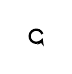
\begin{tikzpicture}[baseline=-0.1ex, scale=0.85]
        % 円環（尾に向かって細くなる円弧）
        \draw[line width=0.8pt, -{Stealth[length=2.8pt, width=2.4pt]}] 
          (20:0.65ex) arc (20:345:0.65ex);
      \end{tikzpicture}%
    }}%
  }%
}
\newcommand{\WholeSelf}{\Ouroboros}

\newcommand{\SixthSense}{\mathscr{N}}

\makeatletter
\newcommand{\dharmawheel}{%
  \mathop{%
    \vcenter{\hbox{%
      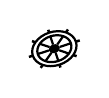
\begin{tikzpicture}[
        baseline=-0.12em, % ← ここをマイナスにして全体を上に持ち上げる（-0.08em 〜 -0.20em で微調整可能）
        line width=0.08em,
        rotate=18, 
        xscale=1.05, yscale=0.78
      ]
        % 外輪（二重楕円）
        \draw[black] (0,0) circle (0.78em);
        \draw[black] (0,0) circle (0.60em);
        
        % 中心軸（ハブ）
        \fill[black] (0,0) circle (0.20em);
        
        % 8本スポーク + 外側ハンドル
        \foreach \angle in {0, 45, 90, 135, 180, 225, 270, 315} {
          \draw[black] (\angle:0.20em) -- (\angle:0.60em);
          \draw[black, line width=0.09em] (\angle:0.78em) -- (\angle:0.92em);
        }
      \end{tikzpicture}%
    }}%
  }\displaylimits
}
\makeatother

\newcommand{\CBO}{\dharmawheel_{\mathrm{CBO}}}

